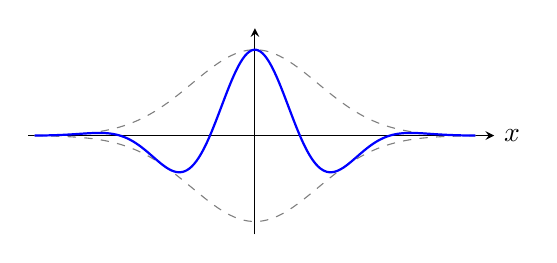
\begin{tikzpicture}
\begin{axis}[width=7.5cm, height=4.2cm, axis lines=middle, xmin=-3.6, xmax=3.8, ymin=-1.15, ymax=1.25,
  xtick=\empty, ytick=\empty, xlabel={$x$}, every axis x label/.style={at={(current axis.right of origin)}, anchor=west},
  clip=false]
\addplot[gray, dashed, domain=-3.5:3.5, samples=100] {exp(-x^2/2)};
\addplot[gray, dashed, domain=-3.5:3.5, samples=100] {-exp(-x^2/2)};
\addplot[blue, thick, domain=-3.5:3.5, samples=200] {exp(-x^2/2)*cos(deg(2.2*x))};
\end{axis}
\end{tikzpicture}
